\section{Introduction}
\label{sec:intro}

Multi-task learning (MTL) fits several related prediction problems together so that problems with few examples can borrow statistical strength from the others \citep{caruana1997multitask, zhang2022survey}. In its linear form, the relationship between tasks is encoded as a regularizer on the matrix of task weights: a trace norm when tasks are believed to share a low-dimensional subspace, an $\ell_{2,1}$ norm when they share a subset of features, or a learned task covariance \citep{argyriou2008convex, obozinski2010joint, zhang2010convex}. These methods are usually evaluated against the opposite extreme, one independent model per task, and the size of the improvement over that baseline is taken as the value of sharing.

There is a second extreme that receives much less attention: a single model fitted to all tasks at once. Multilevel statistics calls the two extremes \emph{no pooling} and \emph{complete pooling}, and the standard recommendation is \emph{partial pooling}, which shrinks each group's estimate towards a common one by an amount learned from the data \citep{gelman2007data}. If tasks share most of their structure, complete pooling can be a strong competitor, and it is strongest precisely where MTL is advertised to help most: when each task has little data.

We study this question on the School benchmark, a set of 139 regression tasks (one per London secondary school) that has served as a standard test of multi-task methods for two decades \citep{bakker2003task, evgeniou2005kernel, argyriou2008convex}. Our study is deliberately small and fully reproducible. It uses one dataset, linear models and squared loss, so that every effect can be traced to a cause. \Cref{fig:overview} previews the central contrast.

On School, the pooled baseline has a mixed record. \citet{evgeniou2005kernel} found that one support vector machine fitted to all schools performed best, ahead of both independent and multi-task kernels, whereas \citet{argyriou2008convex} reported the aggregate model well below multi-task feature learning. Both comparisons use the same, largest training fraction (75\% of each school), where school-specific models are at their strongest. Partial pooling is equally classical: mean-regularized MTL shrinks every task towards a learned common model \citep{evgeniou2004regularized}, and recent theory shows that estimators of this kind adapt to the unknown similarity between tasks, behaving like pooling when tasks are alike and like independent fitting when they are not \citep{duan2023adaptive}. None of these estimators is new. Our contribution is empirical: we measure where on the data-size axis each regime holds on School, and explain why.

\begin{figure}[t]
\centering
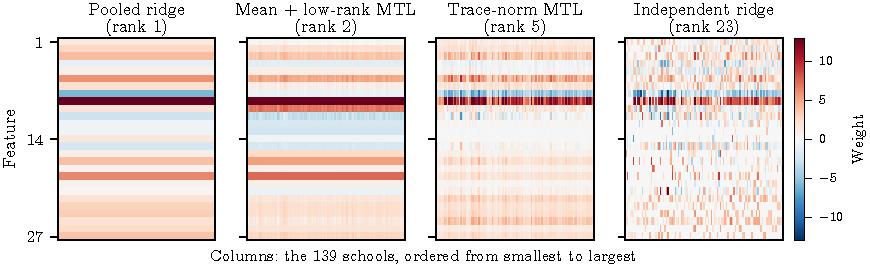
\includegraphics[width=\textwidth]{fig1_model_matrices.pdf}
\caption{Learned model matrices $W$ on School at $\rho = 20\%$ (first split), intercept row omitted; each column is one school's model, schools ordered by size. Pooled ridge uses one model for every school (rank 1), and independent ridge fits each school alone (rank 23). Trace-norm MTL shares a subspace but pales the shared weights, shrinking them towards zero. Mean + low-rank MTL, one of the two partial-pooling estimators we study, keeps the pooled weights and adds small structured deviations.}
\label{fig:overview}
\end{figure}

\paragraph{Contributions.}
\begin{itemize}[leftmargin=*]
\item \textbf{Reproduction.} With a short NumPy implementation of proximal-gradient MTL, we reproduce published School results under two protocols, matching the trace-norm result of \citet{argyriou2008convex} to within 0.2 points of explained variance (\cref{sec:res-repro}).
\item \textbf{Pooling across data sizes.} Over training fractions from 5\% to 75\% of each school, trace-norm MTL beats independent ridge on every split, yet a single pooled ridge model beats it on every split up to 20\% (\cref{sec:res-curves}). We trace this to the data, in which school-level covariates are constant within each school, and to the regularizers, which shrink towards zero rather than towards a common model (\cref{sec:res-why}, \cref{prop:limits}).
\item \textbf{Partial pooling.} Mean-regularized MTL, which learns a shared mean and penalizes only deviations from it, stays within 0.4\% of pooled ridge at 5\% training and is the best or tied-best method from 10\% onwards; constraining the deviations to be low rank does not help (\cref{sec:res-partial}). Its advantage over trace-norm MTL is largest for small schools (\cref{sec:res-who}).
\item \textbf{Evaluation pitfalls.} A fixed iteration budget fails silently on unscaled features, and two common definitions of explained variance differ by 11 to 13 points for identical predictions (\cref{sec:res-optim,sec:res-metrics}).
\end{itemize}
